\chapter{Hyperkinetic movement disorder analysis}
\label{ch:nemo}

\textit{
In this chapter we present a real world application for the dynamic projection methods introduced in \cref{ch:proj-eval,ch:proj-algo} in the context of hyperkinetic movement disorder analysis. These disorders manifest in the form of abnormal involuntary movements that highly affect the quality of life of the people that suffer from them. These involuntary movements may present a wide range of tendencies: they may be regular and rhythmic, as in tremors; swift ``lightning-like'' jerks or twitches, as in myoclonus; sustained and repetitive movements resulting in abnormal postures, as seen in dystonia; they may present a random, brief, and non-rhythmic character, as in chorea; or can be temporarily suppressible jerks, as in tics.
The diagnosis of these disorders is carried out via careful professional observation and can be extra challenging due to the circunstantial emergence of certain behaviours (trigged by a specific postures or tasks) and their manifestation via compound movements, which may include a combination of the various hyperkinesias. All these factors lead to professionals often disagreeing with diagnosis. 
In this chapter we describe how we transform the data collected during clinical experiments to create a powerful reasoning tool using spectral analysis and temporal dimensionality reduction. 
}

\vspace{5mm} %5mm vertical space


\eduardo{This in an initial report, not necesarily what the chapter/paper will look like. It is supposed to help me think about how to write about this project and guide me through preliminary patient data analysis.
\\
In the introduction and initial sections we will need to: \\
1 - introduce hyperkinectic movement disorders \\ 
2 - talk about how their manisfestation in different people can differ wildly and how that makes them challenging to classify/diagnose even for medical especialists. \\
3 - talk about our goals creating this visual exploration tool and how this differs from a more traditional supervised learning approach. \\
\\
What are these goals exactly? And what are the pros/cons over what ziuz is doing (list them here...) 
\\
\\
After that we'll probably need a section introducing the different disorders and possibly explaining how they manifest in some of the tasks for illustration. \\
One thing that I'm not sure about is how familiar we expect the reader to be about these disorders.
\\
Then I think we should start to describe our contribution. And I would start by (1) describing the data itself and all the choices/transformations we make along the way until we get to the dynamic projection. 
\\
This includes: \\
\\
1 - Showing what the RAW data looks like \\
1.1 - General description of the experiment, including the tasks, sensor types, and possibly the different disorders (which must be introduced in a previous section). \\
1.2 - Show 3 axis accelerometer plot for 3 patients (e.g. healthy vs tremor vs chorea) \\
1.3 - Show spectrogram, interpret it, and talk about synchosqueezing \\ 
1.4 - Show how we get that spectrogram into a 'projectable' format: binning of the freqs + sliding window (width, stride) \\
1.5 - Show initial projections --  not sure what data to use here, maybe the 3 patients from before? Probably a more meaningful subset of the data would be better. Right now we have G-PCA, G-tSNE, and PCD-tSNE implemented. Explain dynamic projections and why they are useful and suitable for this application. Maybe do a trail vs single point comparisson.
\\
\\
Next we need to move into data exploration, where we want to find examples of when dynamic projections can bring us insights into the data dynamics and the high dimensional space. Here we will be interested in looking for clusters, outliers, erratic/regular behavior, failures in the data collection, etc.
\\ 
}

\eduardo{CODE: Check code to make sure I can switch sensors (DONE) and that I can 'stack' more than one sensor (NOT DONE))}

\noindent \textbf{Abstract:}

\section{Introduction}

\section{Related work}

\section{Hyperkinectic movement disorders and experiment design}

\section{Our approach (not sure what to call this section)}

Our goal was to design a visual analytics tool that supports the exploration of the motion data generated in the NEMO project. This is important given that the data is vast and has many axes that can be explored: there are over 100 patients, over 30 tasks, and 16 motion units which record accelerometer (3 axes), gyroscope (3 axes), and EMG (1 dimension) at up to 4370 samples per second, plus 3D video, and, for some experiments, page scans. 

Exploring this myriad of data is a challenge in itself, so we aim to provide the medical professionals a tool to effectively navigate and generate useful insights from patient motion patterns. This means our tool must have a few capabilities: we must be able to identify clusters, outliers, erratic observations, failures in the data collection, etc; or thinking in more medical terms, we must be able to compare various hyperkinesias to healthy behaviour, we must be able to identify under which circunstaces certain abnormal tendencies become incident, we must be able to compare the severity and variability of their manisfestation.

Another important aspect is meta analysis, that is, we want to know which combinations of sensors, tasks, patient groups, and preprocessing transformations generate representative data that may be useful in further investigation steps. This is useful if next we want to build a classifier and keep only ``good data'' or if we want to understand what are the minimal resources (sensors and tasks) needed when performing data collection in a third-party clinic.

We envisioned a design that supports Shneiderman's mantra: Overview first, zoom and filter, then details-on-demand. But to generate visualizations and interactions that implement these, we need to perform a series of transformations on the raw data which are explained in detail next (\cref{fig:nemo-pipe}). 

\begin{figure*}[ht]
\centering
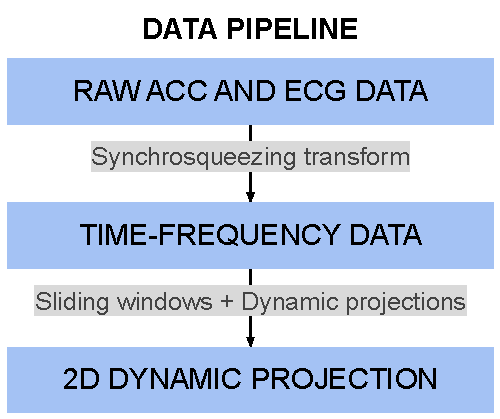
\includegraphics[width=.5\linewidth]{figures/nemo/simple-pipeline.pdf}
\caption{Data transformation pipeline.}
\label{fig:nemo-pipe}
\end{figure*}

To illustrate all the transformations, we begin by inspecting the raw data given by an accelerometer sensor placed on the subjects right hand. The task we will investigate is described as ``Arms stretched forward, wrists straight, palms down, and suppress involuntary movements'' (\cref{fig:hands}).

\begin{figure*}[ht]
\centering
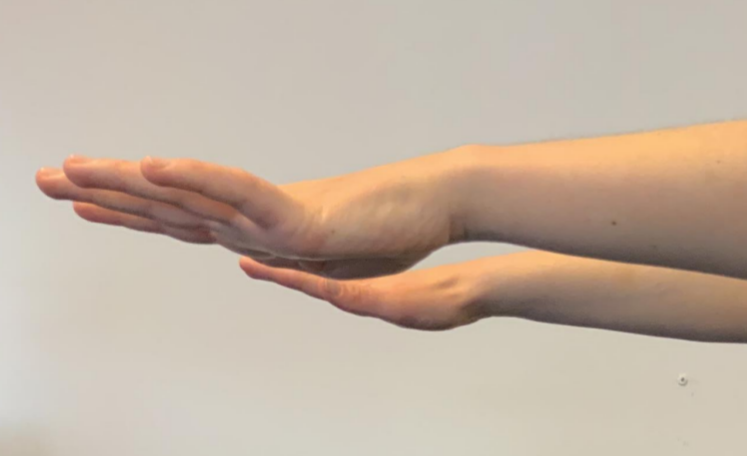
\includegraphics[width=.5\linewidth]{figures/nemo/hands.png}
\caption{Static position with arms and hands streched out in front of body for 20-30 seconds. The subject tries to surpress any involuntary movements.}
\label{fig:hands}
\end{figure*}

\cref{fig:acc} shows the accelerometer data collected during the experiments for three subjects. For each subject we see three colored lines corresponding to the X, Y, and Z axes measurements of a sensor placed on the right opisthenar (back of right the hand) recording at a rate of 148 samples per second. The lines are offset because the sensor is not only reading the subject's movement acceleration, but also the Earth's gravity, as an accelerometer at rest on the surface of the Earth will measure an upwards acceleration due to gravity of $g \approx 9.81 m/s^2$. 

The same sensor unit also records gyroscopic and EMG data. We decided to ignore EMG data for now due to the additional complexity introduced in the non-standard preprocessing steps that (usually) involve noise rejection/filtering, whitening, gain scaling, demodulation, smoothing and relinearization. For the next figures we will only focus on accelerometer data.


On the three subplots of \cref{fig:acc} we see acceleration the data corresponding to three subjects: 
\begin{itemize}
    \item Patient (a) is the healthy control, the lines aren't perfectly straight indicating very low magnitude movement since it's impossible to hold this position perfectly still.
    \item Patient (b)'s measurements show a very rhythmic and regular tremor of average magnitude for the disorder (\eduardo{can anyone check?}). This patient was diagnosed with Essential Tremor, the most common trembling disorder, often confused with Parkinson's disease.
    \item Patient (c) was diagnosed with chorea and displays high amplitude random non-rythmic movements. \eduardo{Are we allowed to upload censored videos to a website?}
\end{itemize}
 

\begin{figure*}[ht]
\centering
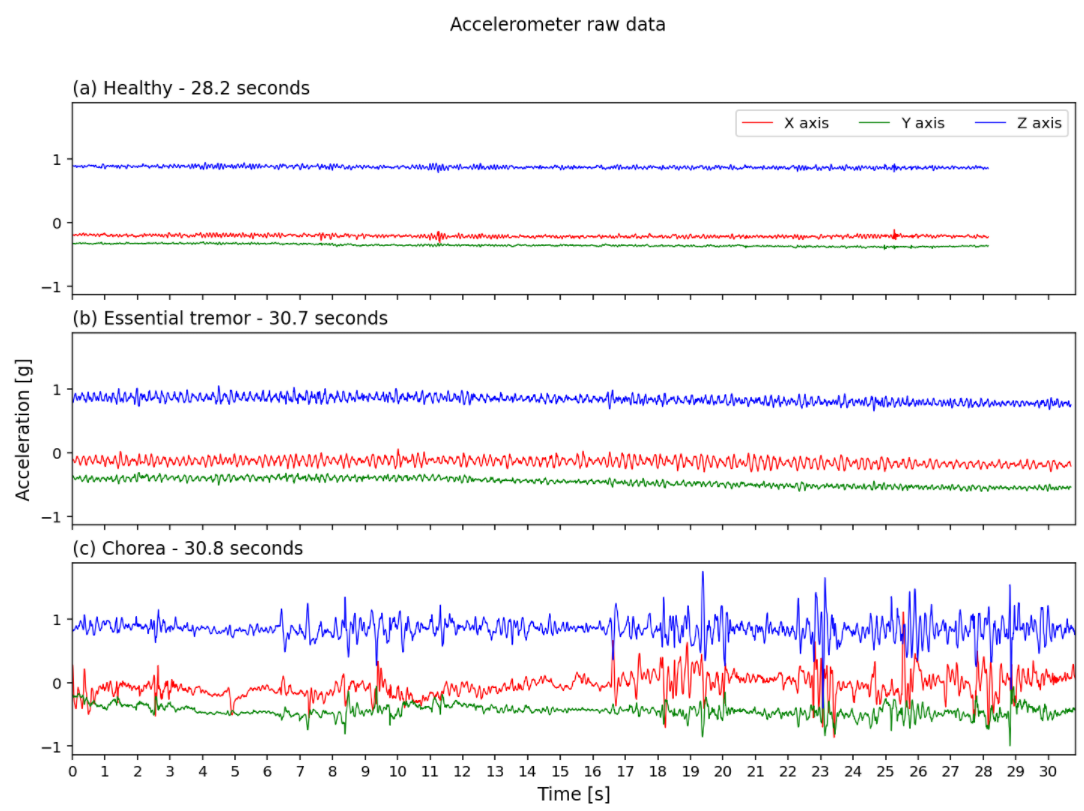
\includegraphics[width=\linewidth]{figures/nemo/acc2.png}
\caption{Accelerometer data for 3 subjects classified by experts as (a) healthy, (b) diagnosed with essential tremor, and (c) diagnosed with chorea. The data corresponds to a task where the subject must hold their hands as still as possible in the position suggested in Fig. \ref{fig:hands}.
Each subplot corresponds to the accelerometer data collected during the experiment and broken down into 3 orthogonal components (X, Y, and Z axis). \eduardo{Are we allowed to upload censored videos to a website?}}
\label{fig:acc}
\end{figure*}


These simple line graphs are very useful for reasoning about the disorders and understanding their behaviour over time. However, they don't tell the full story, as we can get a different perspective on the data that reaveals relevant information hidden in the raw signal by decomposing it into the frequencies that form it. This can be done in two ways: with frequency-domain representation and time-frequency representation. The former assumes that the signal is stationary, which given the nature of our experiments, we know they aren't so we won't be using them. An example of technique used for in this case is the Fourier Transform. In contrast, time-frequency representation allows us to reason about how the the frequency-domain (the spectrum) of a signal changes \textit{over time}.

The technique we use for time-frequency analysis is called Synchrosqueezing Wavelet Transform \eduardo{cite}. It is an improvement over the original Wavelet transform \eduardo{cite} which provides a sparser, sharper, noise-robust, and partly denoised representation of the time-frequency information. \eduardo{how deep do we want to go here?}

This time-frequency representation can be of great relevance for the diagnosis of motion disorders. For example, studies suggest that 95\% of Essential Tremor cases exhibited frequencies in the 5--8Hz range. If we examine \cref{fig:freq}(b), we can see that throught the whole experient, there is a defined presence of frequences in this exact range, showing a regular and insuppressible tendency to the involuntary movement. We don't see the same ``horizontal line'' in that frequency range for patients (a) and (c). Patient (a) is able to hold his/her hand in a much more stable position, which translates into a darker spectrogram (less energy), while patient (c) performs high amplitude random non-rythmic movements characteristic of chorea. The high amplitude can be seen represented by the light colors in the spectrogram, and the ``random non-rythmic'' aspect can be read as having no constant lines in the time-frequecy representation, as seen on patient (b). Having both representations (\cref{fig:acc,fig:freq})side-by-side helps us understand the phenomena as whole. 

The time-frequency representation is especially important because it eases the comparisson of signals. Even though there are methods to compute the similarity between two signals in the time-domain (raw signals) such as RMSE, cross-correlation, and Dynamic Time Warping \eduardo{cite all}, these can be greatly affected by phase shift and small differences in frequency. By doing comparissons in the time-frequency domain, we get a better representation for the next steps of the pipeline.

% https://www.ncbi.nlm.nih.gov/pmc/articles/PMC3475963/


%The sensor reads acceleration in three orthogonal axes (X, Y, Z). For the next figures, we will focus on the Z axis, which points up/down for the hands shown in \cref{fig:hands}.


\begin{figure*}[ht]
\centering
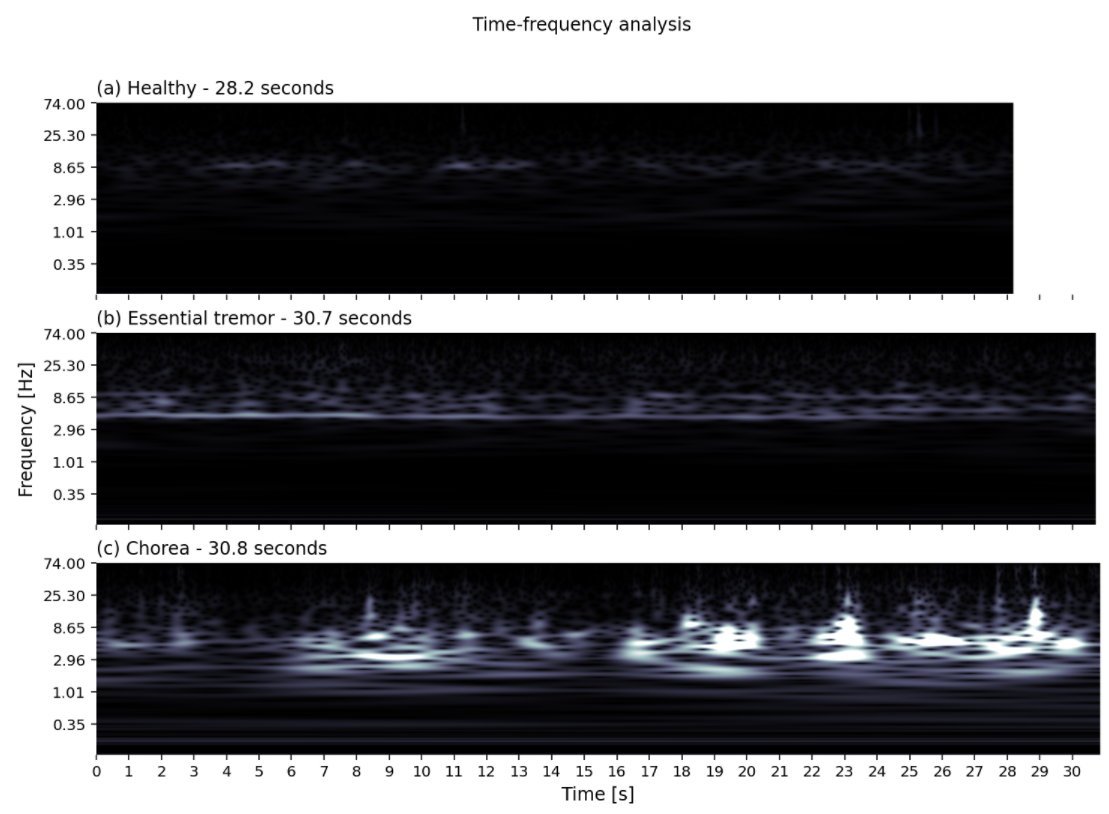
\includegraphics[width=\linewidth]{figures/nemo/freq2.png}
\caption{Time-frequency representation of the acceleration of the Z axis (blue) in Fig. \ref{fig:acc}. Light colors represent high energy in the spectral distribution, i.e., there is a large amplitude component in the subject's movement associated to a particular frequency or frequency distribution. \eduardo{add colormap}}
\label{fig:freq}
\end{figure*}

\begin{figure*}[ht]
\centering
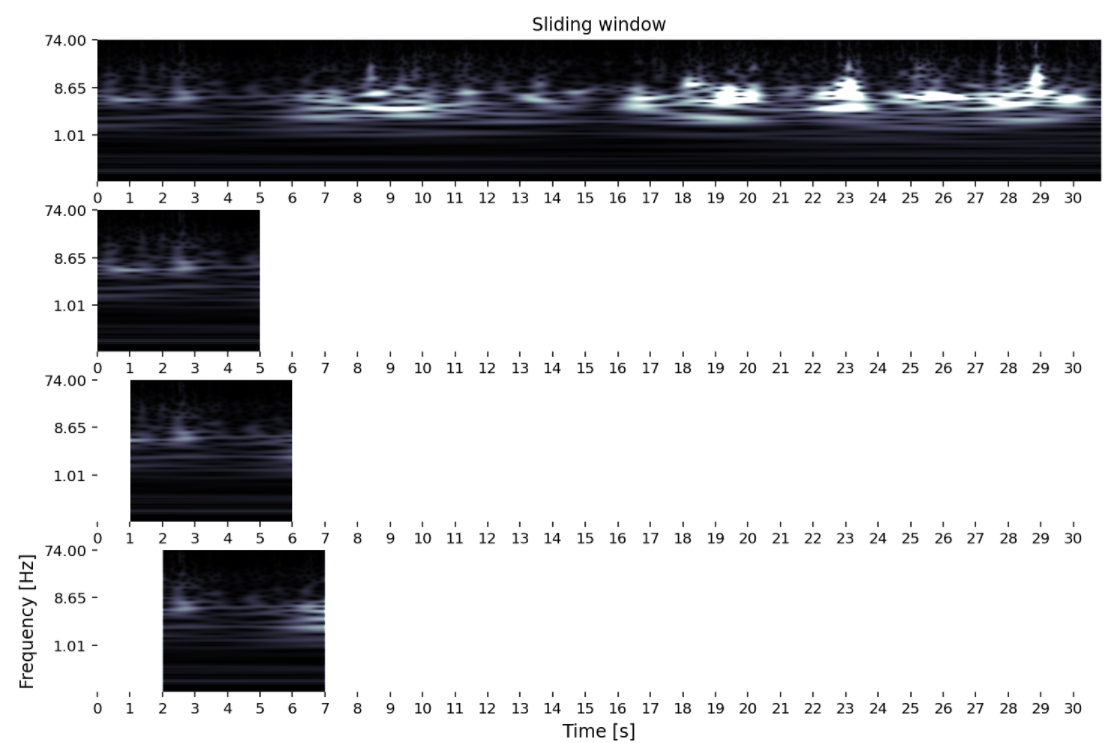
\includegraphics[width=\linewidth]{figures/nemo/sliding.png}
\caption{Before we project our data, we subdivide each spectrogram using the Sliding Window method. In this example, we use a window width of 5 seconds and a stride of 1 second to partition the data from Fig. \ref{fig:freq}c.}
\label{fig:sliding}
\end{figure*}


\begin{figure*}[ht]
\centering
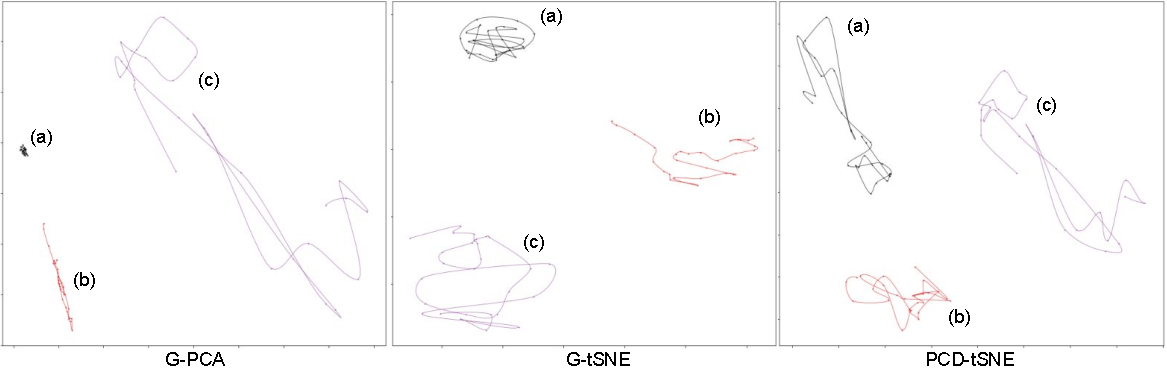
\includegraphics[width=\linewidth]{figures/nemo/nemo1-projections.pdf}
\caption{The last step of the pipeline is to project (using dynamic methods) the data that has been subdivided by the Sliding Window method. Our tool supports 3 dynamic projection methods: G-PCA, G-tSNE, and PCD-tSNE. We visualize the dynamic projections as trails, where we connect the consecutive ``windows''. The data corresponds to the patients presented in \cref{fig:acc,fig:freq}.}
\label{fig:nemo1-projections}
\end{figure*}


\section{Data exploration}

\eduardo{We will limit the analysis to a very small subset of the data (for now). \\
Only one task -- the same as described above --, only one sensor/sensor axis (right hand Z), and only healthy vs tremor patients.} 

\begin{figure}
\centering
\begin{minipage}{.47\textwidth}
    \centering
    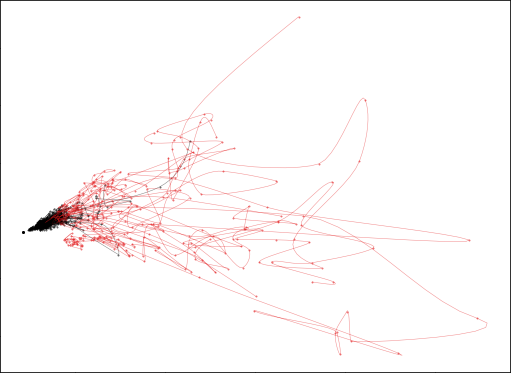
\includegraphics[width=\linewidth]{figures/nemo/exp1.png}
    % \captionof{figure}{A figure}
    \label{fig:exp1-gpca-1s-1s}
\end{minipage}%
\begin{minipage}{.47\textwidth}
    \centering
    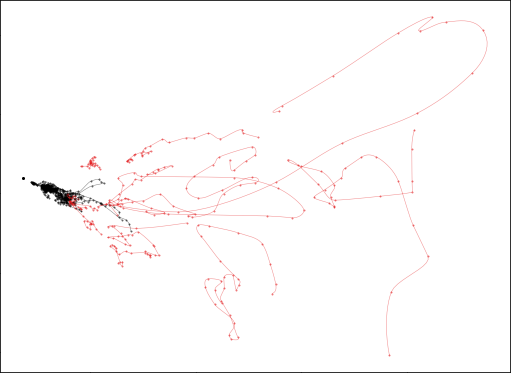
\includegraphics[width=\linewidth]{figures/nemo/exp1-5s-window.png}
    % \captionof{figure}{Another figure}
    \label{fig:exp1-gpca-5s-1s}
\end{minipage}
\caption{G-PCA projection of 24 healthy (black) and 11 tremor (red) patients with window width and stride of [1s, 1s] on the left and [5s, 1s] on the right.}
\end{figure}

\begin{figure*}[ht]
\centering
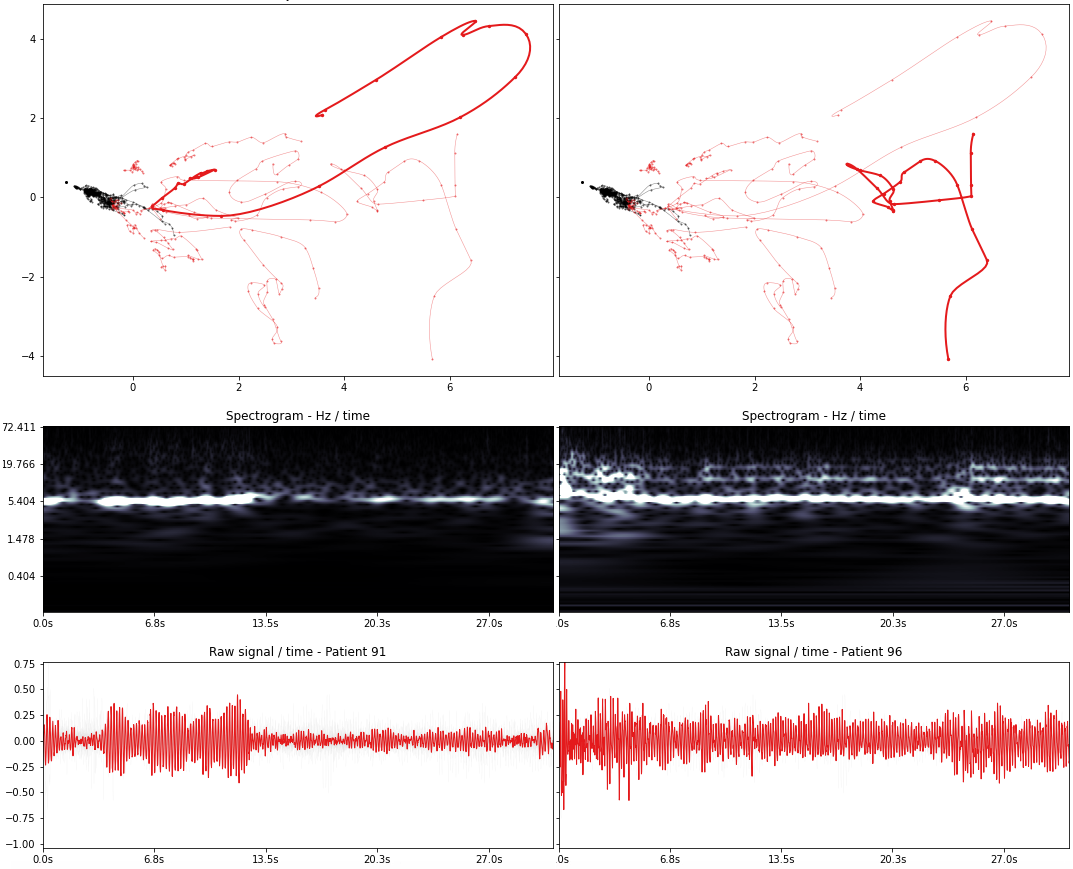
\includegraphics[width=\linewidth]{figures/nemo/exp1-9196.png}
\caption{Our tool allows selection and inspection of patients. Other than the plots shown in the figure, the tool also displays a video recording of the experiment. \eduardo{do we have to hide the patient ids (91 and 96)? }}
\label{fig:exp1-9196}
\end{figure*}

\begin{figure*}[ht]
\centering
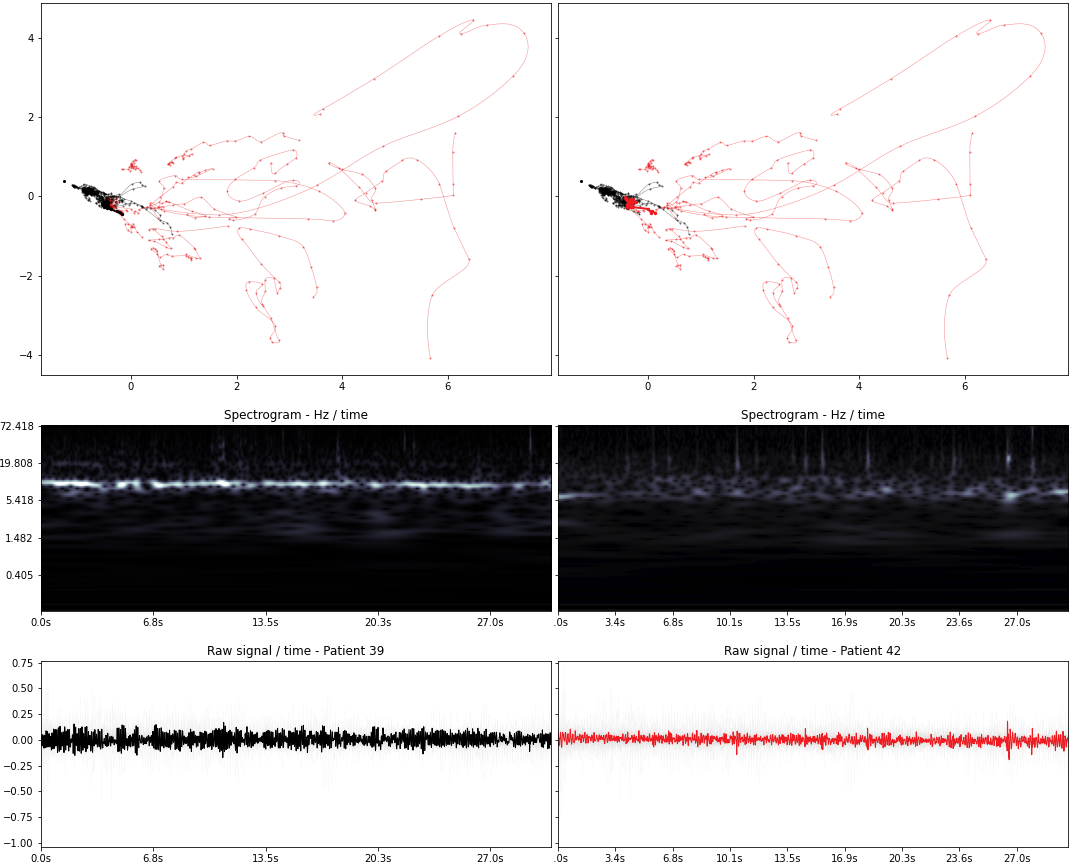
\includegraphics[width=\linewidth]{figures/nemo/exp1-3942.png}
\caption{The trail representing the patient on the right is very close to the healthy group. If we look at only his right hand during the recording of this specific task, it is hard to tell that he/she suffers from tremors and it raises the question as to why was he/she diagnosed with tremors. Does it have a postural aspect to it that isn't captured in this task or perhaps it only appears in certain circunstances?}
\label{fig:exp1-3942}
\end{figure*}

\begin{figure*}[ht]
\centering
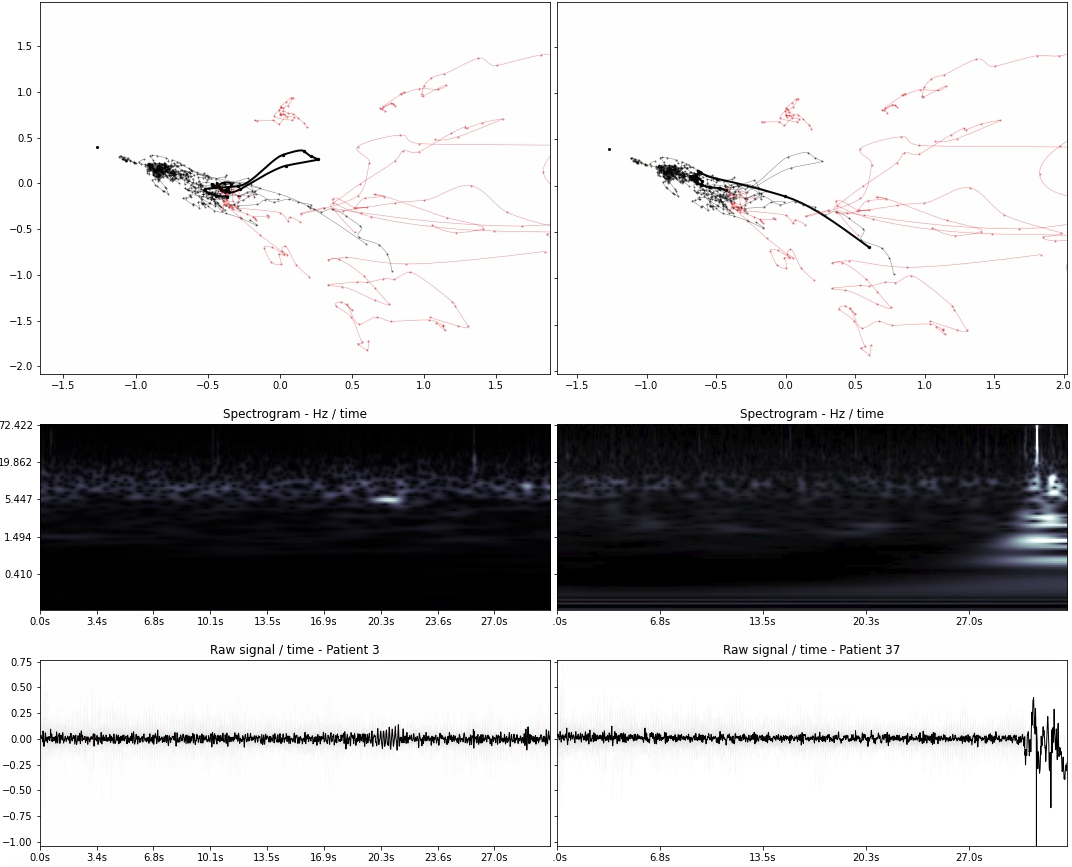
\includegraphics[width=\linewidth]{figures/nemo/exp1-337.png}
\caption{Temporary tremors on the left, and premature end of experiment on the right.}
\label{fig:exp1-337}
\end{figure*}


\begin{figure}
\begin{tabular}{cc}
\subfloat[G-PCA]{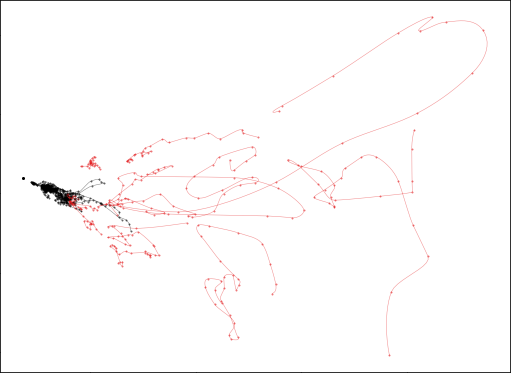
\includegraphics[width=.5\linewidth]{figures/nemo/exp1-5s-window.png}} &
\subfloat[PCD-tSNE $\lambda=.1$]{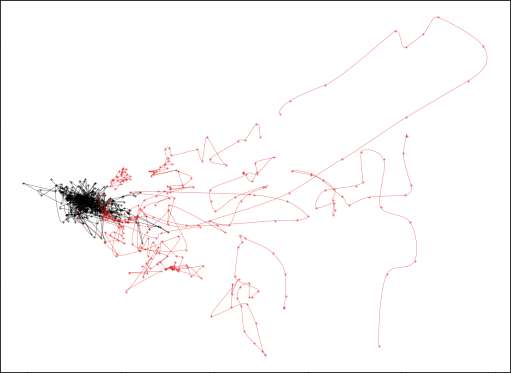
\includegraphics[width=.5\linewidth]{figures/nemo/exp1-pcd0,1.png}} \\
\subfloat[PCD-tSNE $\lambda=.001$]{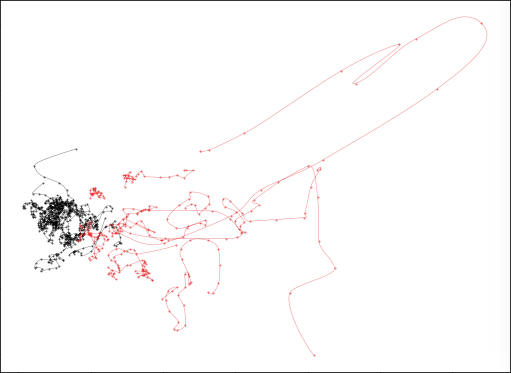
\includegraphics[width=.5\linewidth]{figures/nemo/exp1-pcd0,001.png}} &
\subfloat[PCD-tSNE $\lambda=.0001$]{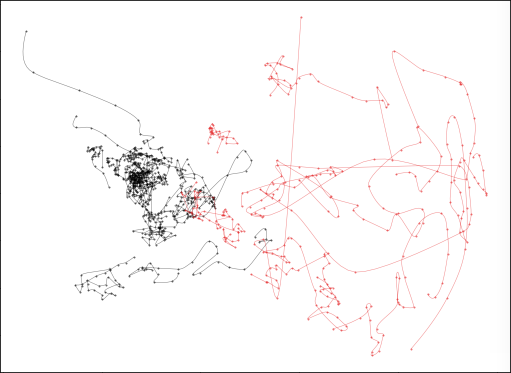
\includegraphics[width=.5\linewidth]{figures/nemo/exp1-pcd0,0001.png}}\\
\subfloat[PCD-tSNE $\lambda=.000001$]{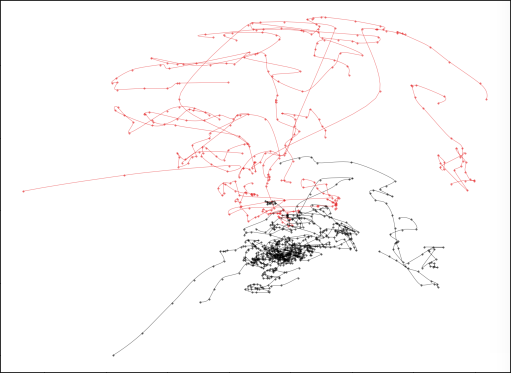
\includegraphics[width=.5\linewidth]{figures/nemo/exp1-pcd0,000001.png}} &
\subfloat[G-tSNE]{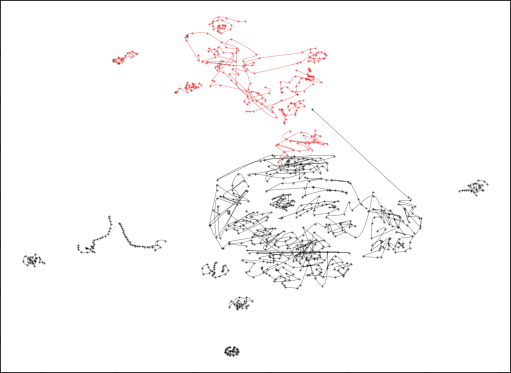
\includegraphics[width=.5\linewidth]{figures/nemo/exp1-gtsne.png}}
\end{tabular}
\caption{}
\end{figure}


\section{Discussion}

% right now we are only doing task-wise analysis, maybe we want to change the focus to the analysis of a given patient given what we know is normal and abnormal behaviour.

\section{Conclusions}


    
